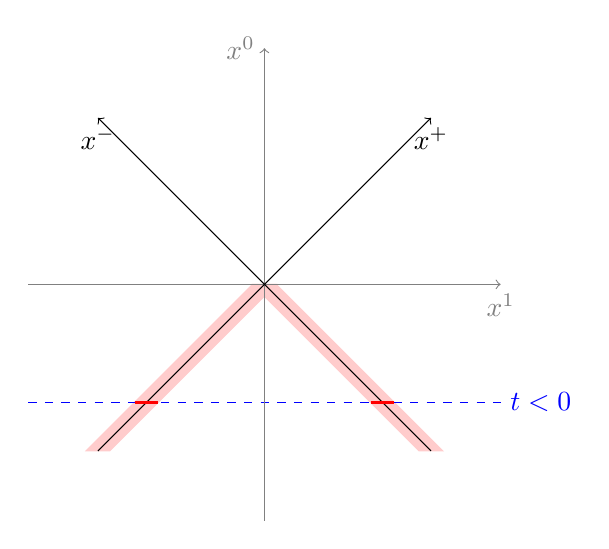
\begin{tikzpicture}[scale = 1.5]
	%trajectories
	\filldraw[red!20!white] (-1.51,-1.41) -- (-0.1,0) -- (0.1,0) -- (-1.31,-1.41) -- cycle;
	\filldraw[red!20!white] (1.51,-1.41) -- (0.1,0) -- (-0.1,0) -- (1.31,-1.41) -- cycle;
	%present line
	\draw[blue,dashed] (-2,-1) -- (2,-1) node[right] {$t<0$};
	%axes
	\draw[->,gray] (-2,0) -- (2,0) node[below] {$x^1$};
	\draw[->,gray] (0,-2) -- (0,2) node[left] {$x^0$};
	\draw[->] (1.41,-1.41) -- (-1.41,1.41) node[below] {$x^-$};
	\draw[->] (-1.41,-1.41) -- (1.41,1.41) node[below] {$x^+$};
	%nuclei
	\draw[red,very thick] (-1.1,-1) -- (-0.9,-1);
	\draw[red,very thick] (0.9,-1) -- (1.1,-1);
	%text
\end{tikzpicture}
